\documentclass[tikz]{standalone}
\usepackage{tikz}
\usetikzlibrary{arrows.meta, shapes.arrows, positioning}

\begin{document}
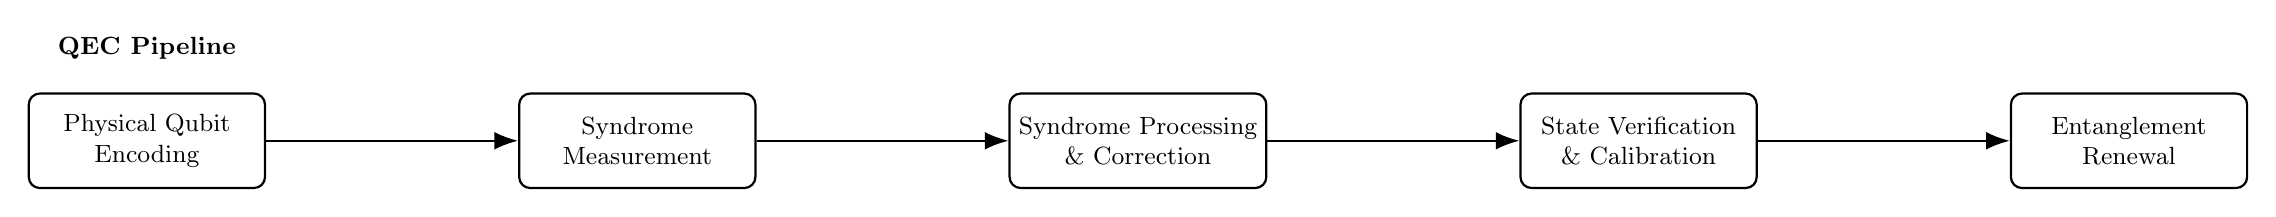
\begin{tikzpicture}[font=\small, 
  stage/.style={
    thick,
    draw,
    rectangle,
    minimum width=3.0cm,
    minimum height=1.2cm,
    align=center,
    rounded corners
  },
  line/.style={-{Latex[length=3mm]}, thick},
  node distance=3.2cm
  ]

% Pipeline stages
\node[stage] (encode) {Physical Qubit\\Encoding};
\node[stage, right=of encode] (synd_meas) {Syndrome\\Measurement};
\node[stage, right=of synd_meas] (proc_corr) {Syndrome Processing\\\& Correction};
\node[stage, right=of proc_corr] (verify) {State Verification\\\& Calibration};
\node[stage, right=of verify] (renew) {Entanglement\\Renewal};

% Arrows
\draw[line] (encode) -- (synd_meas);
\draw[line] (synd_meas) -- (proc_corr);
\draw[line] (proc_corr) -- (verify);
\draw[line] (verify) -- (renew);

% Optional: label the pipeline
\node[above=0.3cm of encode] {\textbf{QEC Pipeline}};

\end{tikzpicture}
\end{document}
